\documentclass{article}
\usepackage{amsmath}
\usepackage{amssymb}
\usepackage{graphicx}
\usepackage{tikz}
\usepackage{pgfplots}
\usetikzlibrary{plotmarks}

\title{Comprehensive Study of Algebra 2 Concepts}
\author{Badger Code}
\date{\today}

\begin{document}
\maketitle

\section{Polynomials and Factoring}
Polynomials are expressions consisting of variables and coefficients combined using addition, subtraction, and multiplication operations. Factoring involves breaking down polynomials into simpler terms.

\subsection{Polynomial Operations}
Consider the polynomial $P(x) = 2x^3 - 5x^2 + 3x - 7$. To simplify, perform operations:
\begin{align*}
    P(x) + 4x^2 &= 2x^3 - x^2 + 3x - 7 + 4x^2 \\
    &= 2x^3 + 3x - 7 + 3x^2 \\
    &= 2x^3 + 3x^2 + 3x - 7
\end{align*}

\subsection{Factoring Techniques}
Let's factor the quadratic polynomial $Q(x) = x^2 - 4x + 4$. We use the difference of squares pattern:
\begin{align*}
    Q(x) &= x^2 - 4x + 4 \\
    &= x^2 - 2 \cdot 2x + 2^2 \\
    &= (x - 2)^2
\end{align*}

\section{Rational Expressions}
Rational expressions are ratios of two polynomials. They can be added, subtracted, multiplied, and divided.

\subsection{Simplifying Rational Expressions}
Consider the rational expression $R(x) = \frac{3x^2 + 6x}{2x^2 - x - 6}$. To simplify, factor the polynomials:
\begin{align*}
    R(x) &= \frac{3x(x + 2)}{(2x + 3)(x - 2)} \\
    &= \frac{3x(x + 2)}{(x + 2)(2x - 3)}
\end{align*}

\subsection{Adding and Subtracting Rational Expressions}
Let's add the rational expressions $S(x) = \frac{x}{x + 1} + \frac{2}{x + 1}$:
\begin{align*}
    S(x) &= \frac{x + 2}{x + 1}
\end{align*}

% Include a graph using TikZ
\subsection{Graphing Quadratic Functions}
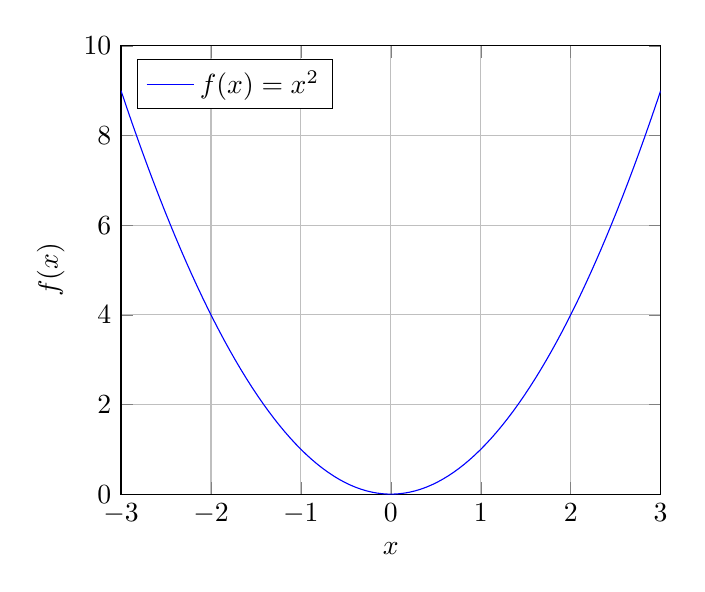
\begin{tikzpicture}
    \begin{axis}[
        xlabel=$x$,
        ylabel=$f(x)$,
        xmin=-3, xmax=3,
        ymin=0, ymax=10,
        grid=both,
        xtick={-3, -2, ..., 3},
        ytick={0, 2, ..., 10},
        legend pos=north west,
    ]
    \addplot[blue, samples=100, domain=-3:3]{x^2};
    \legend{$f(x) = x^2$}
    \end{axis}
\end{tikzpicture}

\section{Quadratic Functions and Equations}
Quadratic functions are characterized by the highest power of the variable being 2. They often form a parabolic shape.

\subsection{Vertex Form and Completing the Square}
Consider the quadratic function $f(x) = x^2 - 4x + 3$. To find the vertex, complete the square:
\begin{align*}
    f(x) &= x^2 - 4x + 3 \\
    &= (x - 2)^2 - 1
\end{align*}
The vertex is $(2, -1)$.

\subsection{Quadratic Formula}
To solve the quadratic equation $x^2 - 5x + 6 = 0$, use the quadratic formula:
\begin{align*}
    x &= \frac{-b \pm \sqrt{b^2 - 4ac}}{2a} \\
    &= \frac{5 \pm \sqrt{25 - 24}}{2} \\
    &= \frac{5 \pm 1}{2} \\
    &= 3 \text{ or } 2
\end{align*}

\section{Exponential and Logarithmic Functions}
Exponential functions involve a constant base raised to a variable exponent. Logarithmic functions are the inverses of exponential functions.

\subsection{Exponential Growth and Decay}
The formula for exponential growth/decay is given by $A(t) = A_0 e^{kt}$, where $A_0$ is the initial amount, $k$ is the growth/decay rate, and $t$ is time.

\subsection{Solving Logarithmic Equations}
Solve the logarithmic equation $\log_2(x + 3) = 4$:
\begin{align*}
    x + 3 &= 2^4 \\
    x &= 16 - 3 \\
    x &= 13
\end{align*}

\section{Conic Sections}
Conic sections are formed by intersecting a plane with a double-napped cone. They include the circle, ellipse, parabola, and hyperbola.

\subsection{Equation of a Circle}
The equation of a circle with center $(h, k)$ and radius $r$ is:
\[ (x - h)^2 + (y - k)^2 = r^2 \]

\subsection{Graphing an Ellipse}
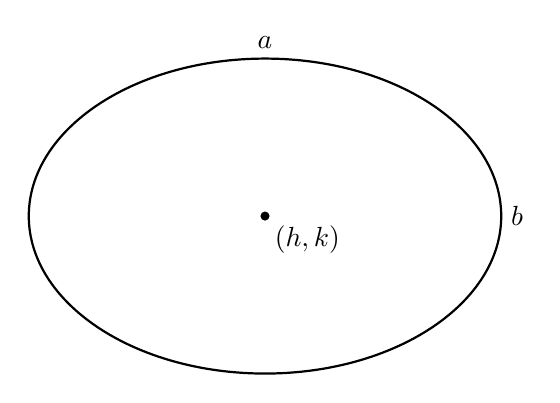
\begin{tikzpicture}
    \draw[thick] (0, 0) ellipse (3 and 2);
    \draw[fill] (0, 0) circle [radius=0.05];
    \node[above] at (0, 2) {$a$};
    \node[right] at (3, 0) {$b$};
    \node[below right] at (0, 0) {$(h, k)$};
\end{tikzpicture}

\section{Systems of Equations and Inequalities}
A system of equations involves multiple equations with the same variables. Solutions are the values that satisfy all the equations.

\subsection{Solving a Linear System}
Solve the system:
\begin{align*}
    2x + 3y &= 8 \\
    4x - y &= 7
\end{align*}
By elimination:
\begin{align*}
    2x + 3y &= 8 \\
    8x - 2y &= 28
\end{align*}
Subtracting the equations gives $6x + 5y = -20$. Solving for $y$, $y = -\frac{6x + 20}{5}$. Substituting into the second equation, $4x + \frac{6x + 20}{5} = 7$. Solving for $x$, $x = 2$. Substituting into $2x + 3y = 8$, $y = \frac{2}{3}$. So, the solution is $x = 2$, $y = \frac{2}{3}$.

\section{Matrices and Determinants}
Matrices are arrays of numbers. Determinants are scalar values associated with square matrices.

\subsection{Matrix Operations}
Given matrices $A = \begin{bmatrix} 2 & 3 \\ 1 & 4 \end{bmatrix}$ and $B = \begin{bmatrix} 5 & 2 \\ 3 & 1 \end{bmatrix}$, calculate $AB$:
\begin{align*}
    AB &= \begin{bmatrix} 2 \cdot 5 + 3 \cdot 3 & 2 \cdot 2 + 3 \cdot 1 \\ 1 \cdot 5 + 4 \cdot 3 & 1 \cdot 2 + 4 \cdot 1 \end{bmatrix} \\
    &= \begin{bmatrix} 19 & 8 \\ 17 & 6 \end{bmatrix}
\end{align*}

\subsection{Determinants and Inverses}
The determinant of a $2 \times 2$ matrix $\begin{bmatrix} a & b \\ c & d \end{bmatrix}$ is $ad - bc$. If the determinant is non-zero, the matrix has an inverse given by:
\[ A^{-1} = \frac{1}{ad - bc} \begin{bmatrix} d & -b \\ -c & a \end{bmatrix} \]

\section{Probability and Statistics}
Probability deals with the likelihood of events occurring. Statistics involves collecting, analyzing, interpreting, and presenting data.

\subsection{Measures of Central Tendency}
The mean (average), median (middle value), and mode (most frequent value) are measures of central tendency used to describe data.

\subsection{Probability Distributions}
Probability distributions describe the likelihood of different outcomes in a random experiment. Discrete distributions include the binomial and Poisson distributions. Continuous distributions include the normal distribution.

\subsection{Statistical Analysis}
Statistical analysis involves methods like hypothesis testing, confidence intervals, and regression analysis to make inferences and predictions from data.

\section{Trigonometry}
Trigonometry deals with the relationships between angles and sides in triangles.

\subsection{Trigonometric Ratios}
In a right triangle, the primary trigonometric ratios are defined as follows:
\begin{align*}
    \sin(\theta) &= \frac{\text{opposite}}{\text{hypotenuse}} \\
    \cos(\theta) &= \frac{\text{adjacent}}{\text{hypotenuse}} \\
    \tan(\theta) &= \frac{\text{opposite}}{\text{adjacent}}
\end{align*}

\subsection{Trigonometric Identities}
Trigonometric identities are equations involving trigonometric functions that hold true for all values of the variables.

\subsection{Graphing Trigonometric Functions}
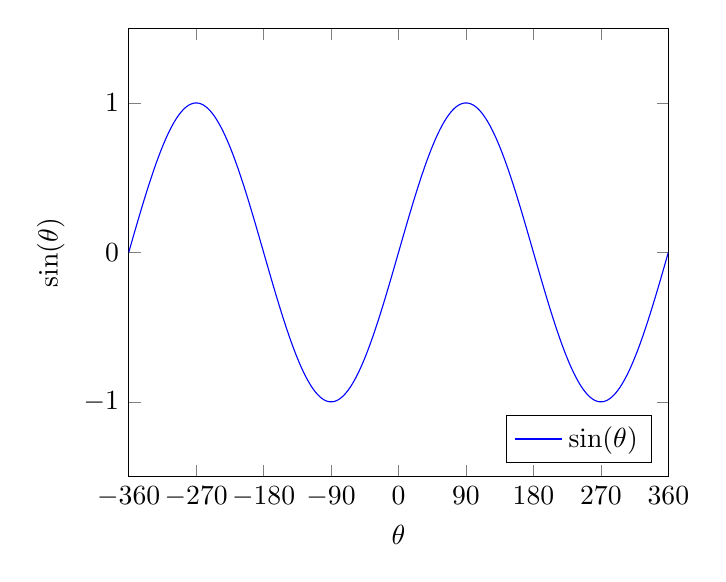
\begin{tikzpicture}
    \begin{axis}[
        xlabel=$\theta$,
        ylabel=$\sin(\theta)$,
        xmin=-360, xmax=360,
        ymin=-1.5, ymax=1.5,
        xtick={-360, -270, ..., 360},
        ytick={-1, 0, 1},
        legend pos=south east,
    ]
    \addplot[blue, samples=400, domain=-360:360]{sin(x)};
    \legend{$\sin(\theta)$}
    \end{axis}
\end{tikzpicture}

\section{Conclusion}
Algebra 2 concepts encompass a diverse range of mathematical ideas. From polynomials and factoring to trigonometry and statistics, these concepts provide a foundational understanding of algebraic principles. This paper has offered in-depth explanations, numerous examples, and visual aids to enhance your grasp of Algebra 2.

\end{document}